
\subsection{Generating the User Profile}
Social media's effect on the world is something significant~\cite{Miller2016}.
That is why this application builds a user profile from
the user's social media. 

The application built by Lim et al.~\cite{Lim2018a} allowed the user to connect
the application with their Flickr profile to scan their past trips. However,
Facebook provides an API that would allow users to connect both their Facebook
and Instagram accounts and request content from the user with their permission.
A significant advantage is that the API allows the
application not to limit the results to mimic only
past user's trips like the application by Lim et al.~\cite{Lim2018a} and gather
preferences from his complete profile.
The app requests two things from the
potential tourist's social media, the photos and the liked pages and tries to
classify these into six categories that make up the user's travel interest
vector; 

\begin{center}
    [   
    1 Beach,
    2 Nature,
    3 Shopping,
    4 Museums,
    5 Clubbing,
    6 Bars ]
    
\end{center}



These categories are the same categories that we requested from the google maps
API except `cafeterias' and `restaurants'. These two categories were not
included because the application tries to suggest the best places to eat as
part of the timetable, irrelevant to the user's profile. At the start of the
application, the app initialises all vector values to zero and increments a
value whenever the user's content matches a category. We will describe how the
app classifies both the user's liked pages and the user's photos separately in
the upcoming subsections.

\subsubsection{Transforming the liked pages into the travel interest vector}

The Facebook API allows the application to request each category of the user's
liked Facebook pages. The API's documentation contains a whole list of possible
categories. 
%TODO: Add Url
%https://www.facebook.com/pages/category. 

The app iterates through
all of these user's likes categories and increments a value in the user's
vector whenever the Facebook result matches one of the six travel interest
vector values. For example, if a user likes a page with class `DJ', the user's
clubbing vector value is incremented, and if a page is labelled as a
`Mountain', the app increments the user's nature vector value.

\subsubsection{Transforming the user's photos into the travel interest vector}


Convolutional Neural Networks have become a standard
for classifying an image because of their high
accuracy~\cite{Zhou2018}. Therefore, we decided to test
out two approaches for classifying the photos into the
app's six categories. 

Zhou et al. \cite{Zhou2018} trained several CNNs for
scene recognition and generic deep scene features for
visual identification. However, the places365 models
are not explicitly trained on the six categories of
our application. Therefore, we need to carefully map
the 365 categories with our six application's
categories. That is why we introduced a Tensorflow
Keras sequential model, explicitly trained on the six
application's categories to compare.

\paragraph{Pretrained Places365 models:} These models
are trained on the places365-standard dataset of about
1.8 million images to classify an image into 365
different scene categories. We used the Resnet
places365 models, Resnet-18 and Resnet-50 since they
achieved the highest top-5 validation accuracy on the
places365 dataset. The Resnet 18 comprises 18, and the
Resnet 50 comprises 50 convolutional layers. They both
converge to an output layer representing the 365
output categories.  Figure \ref{Resnet} shows a
summary of the whole Resnet 18 model.

\paragraph{Trained Tensorflow Keras model: } This
model contains three convolutional layers with a
rectified linear unit (ReLu) activation function. A
pooling layer follows each to lower the input volume's
spatial dimension for the upcoming layers. The first
layer is a rescaling layer that resizes an image to
180$\times$180 pixels. The final layer represents a
flattening layer and two dense layers to reduce the
outputs to the six application categories, and another
representing the `None' classification. Figure
~\ref{Keras} shows a summary of the whole model.

\begin{figure}[h]
\centering
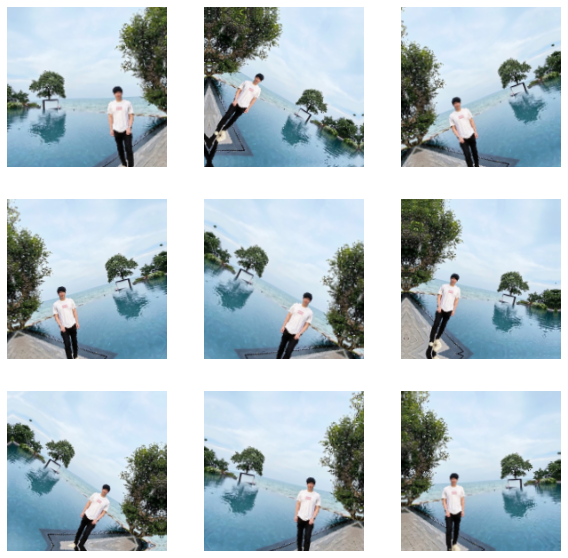
\includegraphics[width=0.3\textwidth]{Augmentation.png}
\caption{Data augmentation to reduce overfitting}
\label{Augmentation}
\end{figure}

The dataset contains 3600 public internet images
representing the seven classes: Beach, Nature,
Museums, Shopping, Clubbing and Bars and None. The
tensor library provides tools to Split the dataset
into a training and validation set Distribute the
photos into batches of 32 Cache the dataset to memory
to prevent I/O blocking All of the images were resized
to 180x180 pixels, and the RGB values were normalised
from zero to one.  	Since the dataset is small
compared to the places 365 models, the training
process is prone to overfitting. Data augmentation
generates additional samples using random
transformations on the dataset. Figure \ref{Augmentation} shows an
example of data augmentation on a photo. We also added
a dropout layer to the model randomly drops sets the
input values of the neuron. These two techniques help
the model avoid overfitting.


\begin{figure}[H]
  \centering
  \begin{minipage}[b]{0.4\textwidth}
    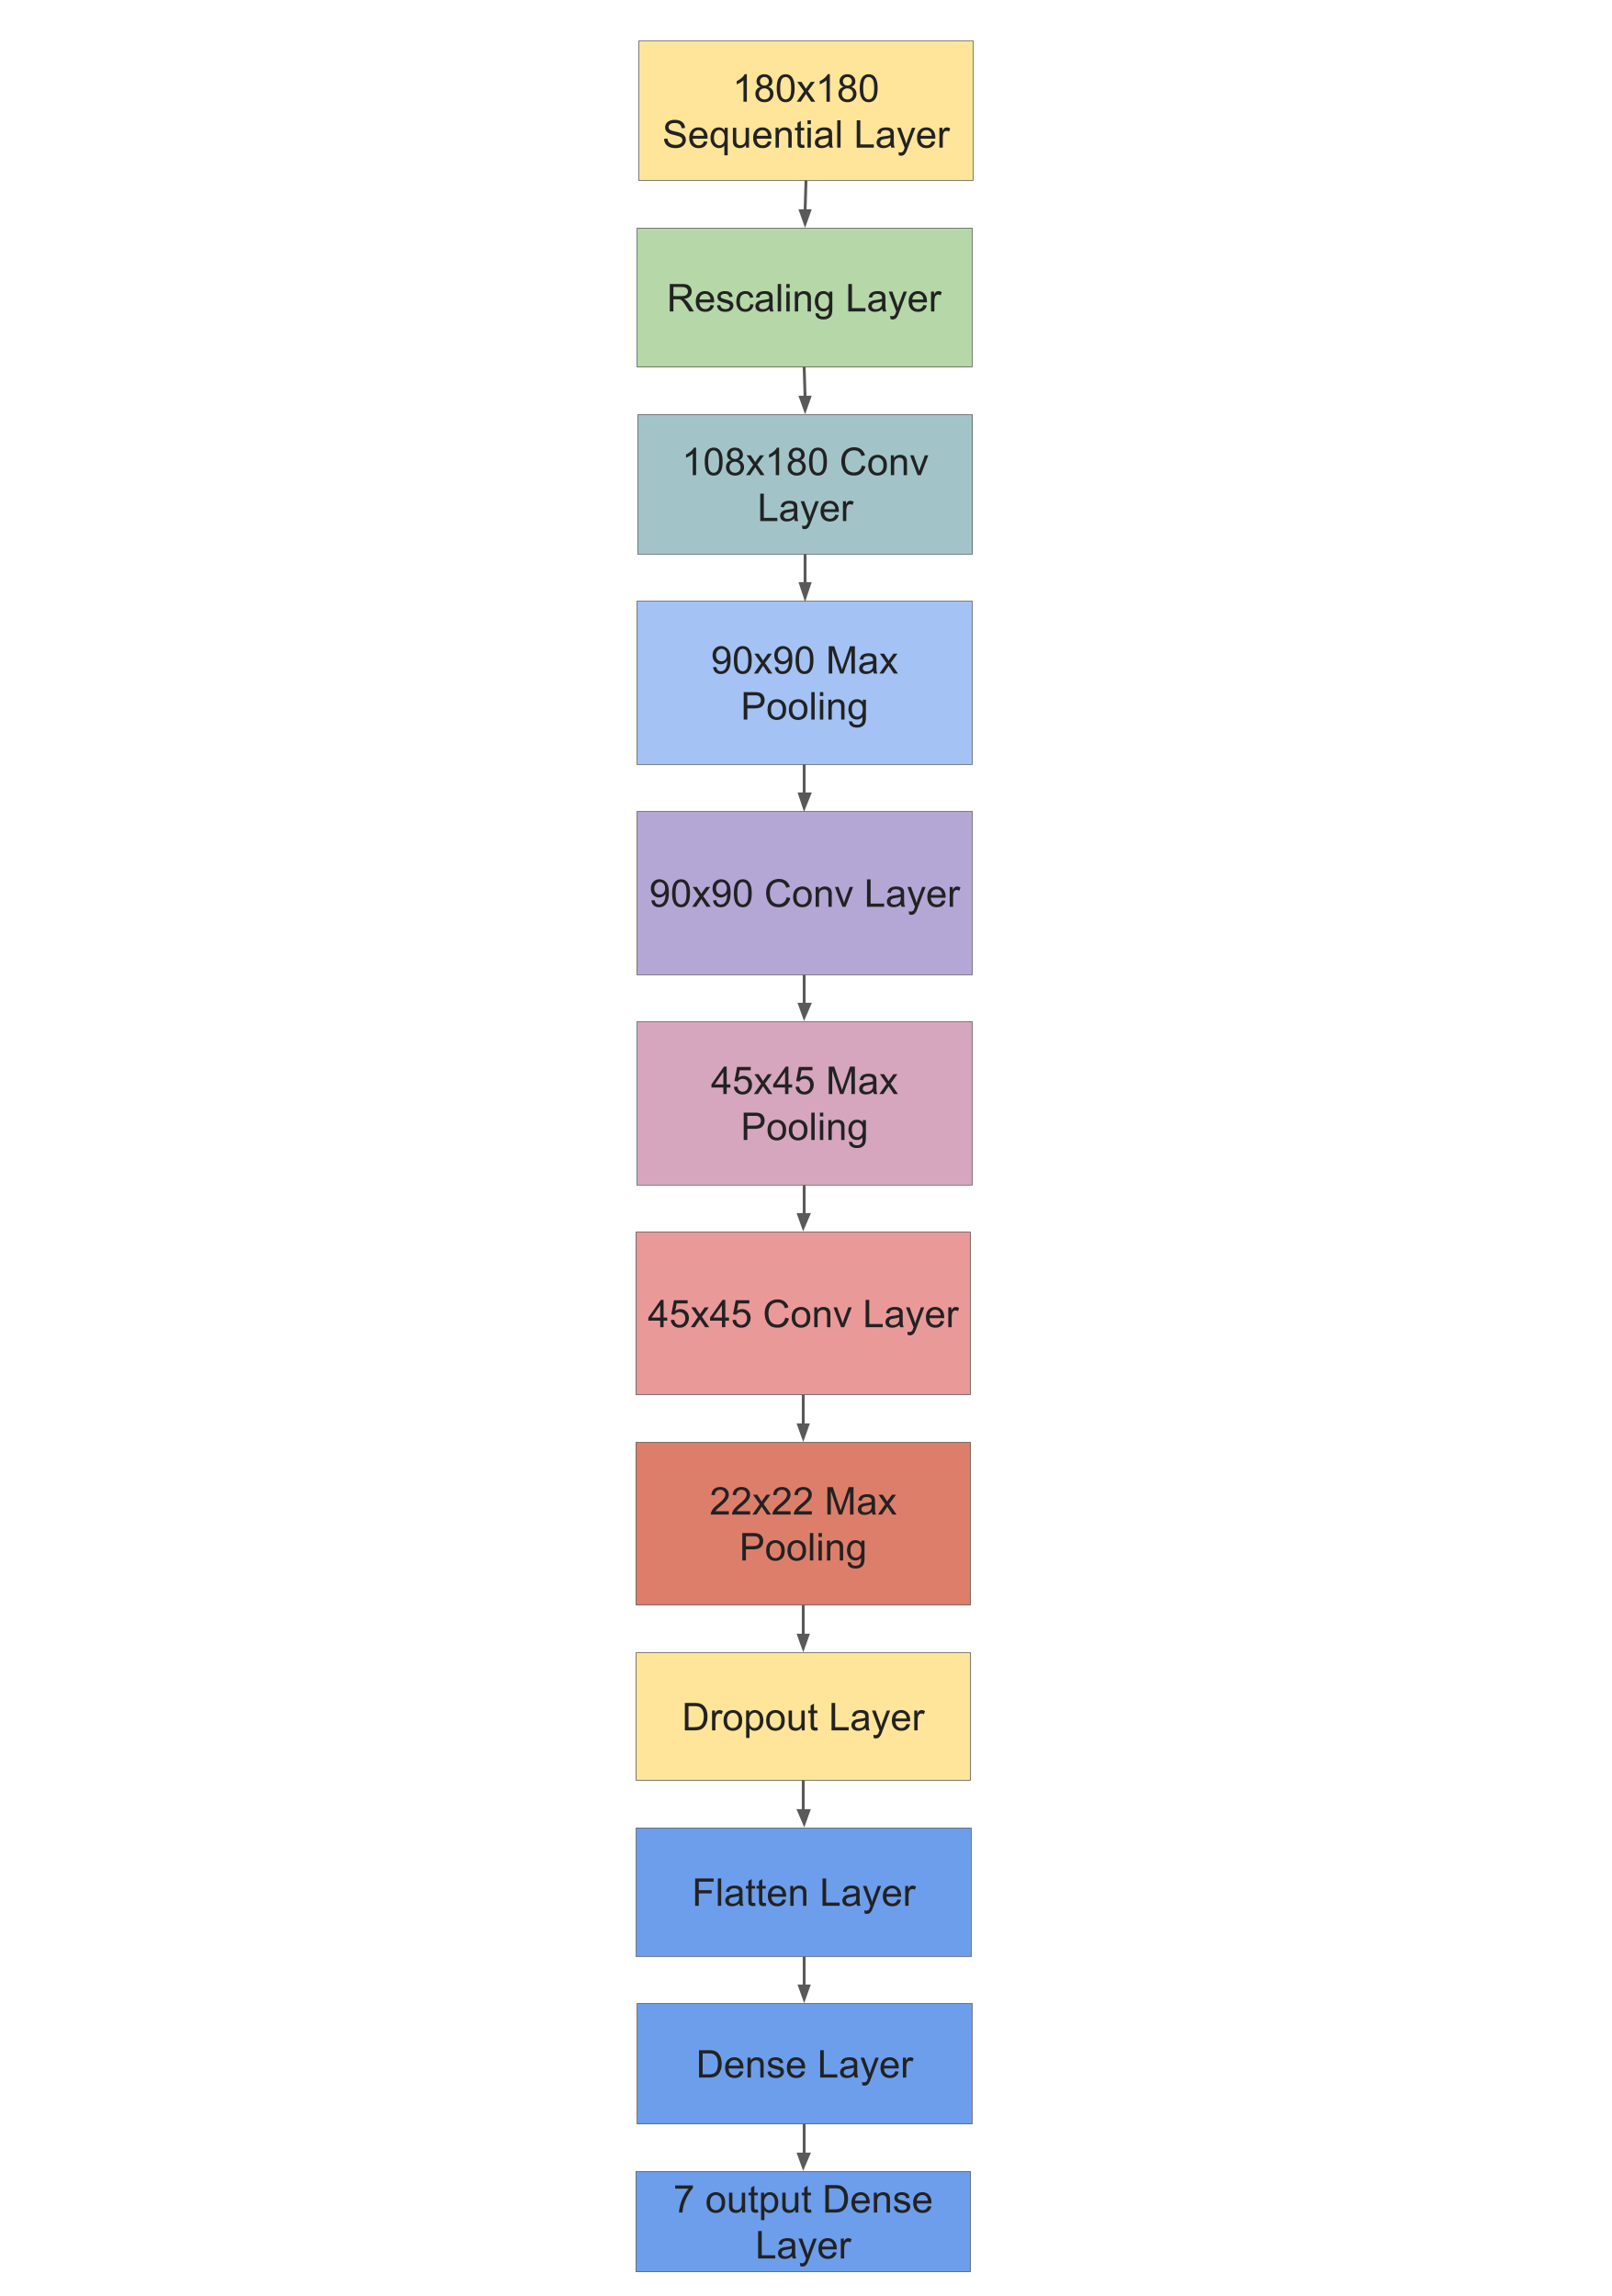
\includegraphics[width=0.8\textwidth]{KerasSequential.png}
    \caption{Keras Sequential Architecture Summary}
    \label{Keras}
  \end{minipage}
  \hfill
  \begin{minipage}[b]{0.4\textwidth}
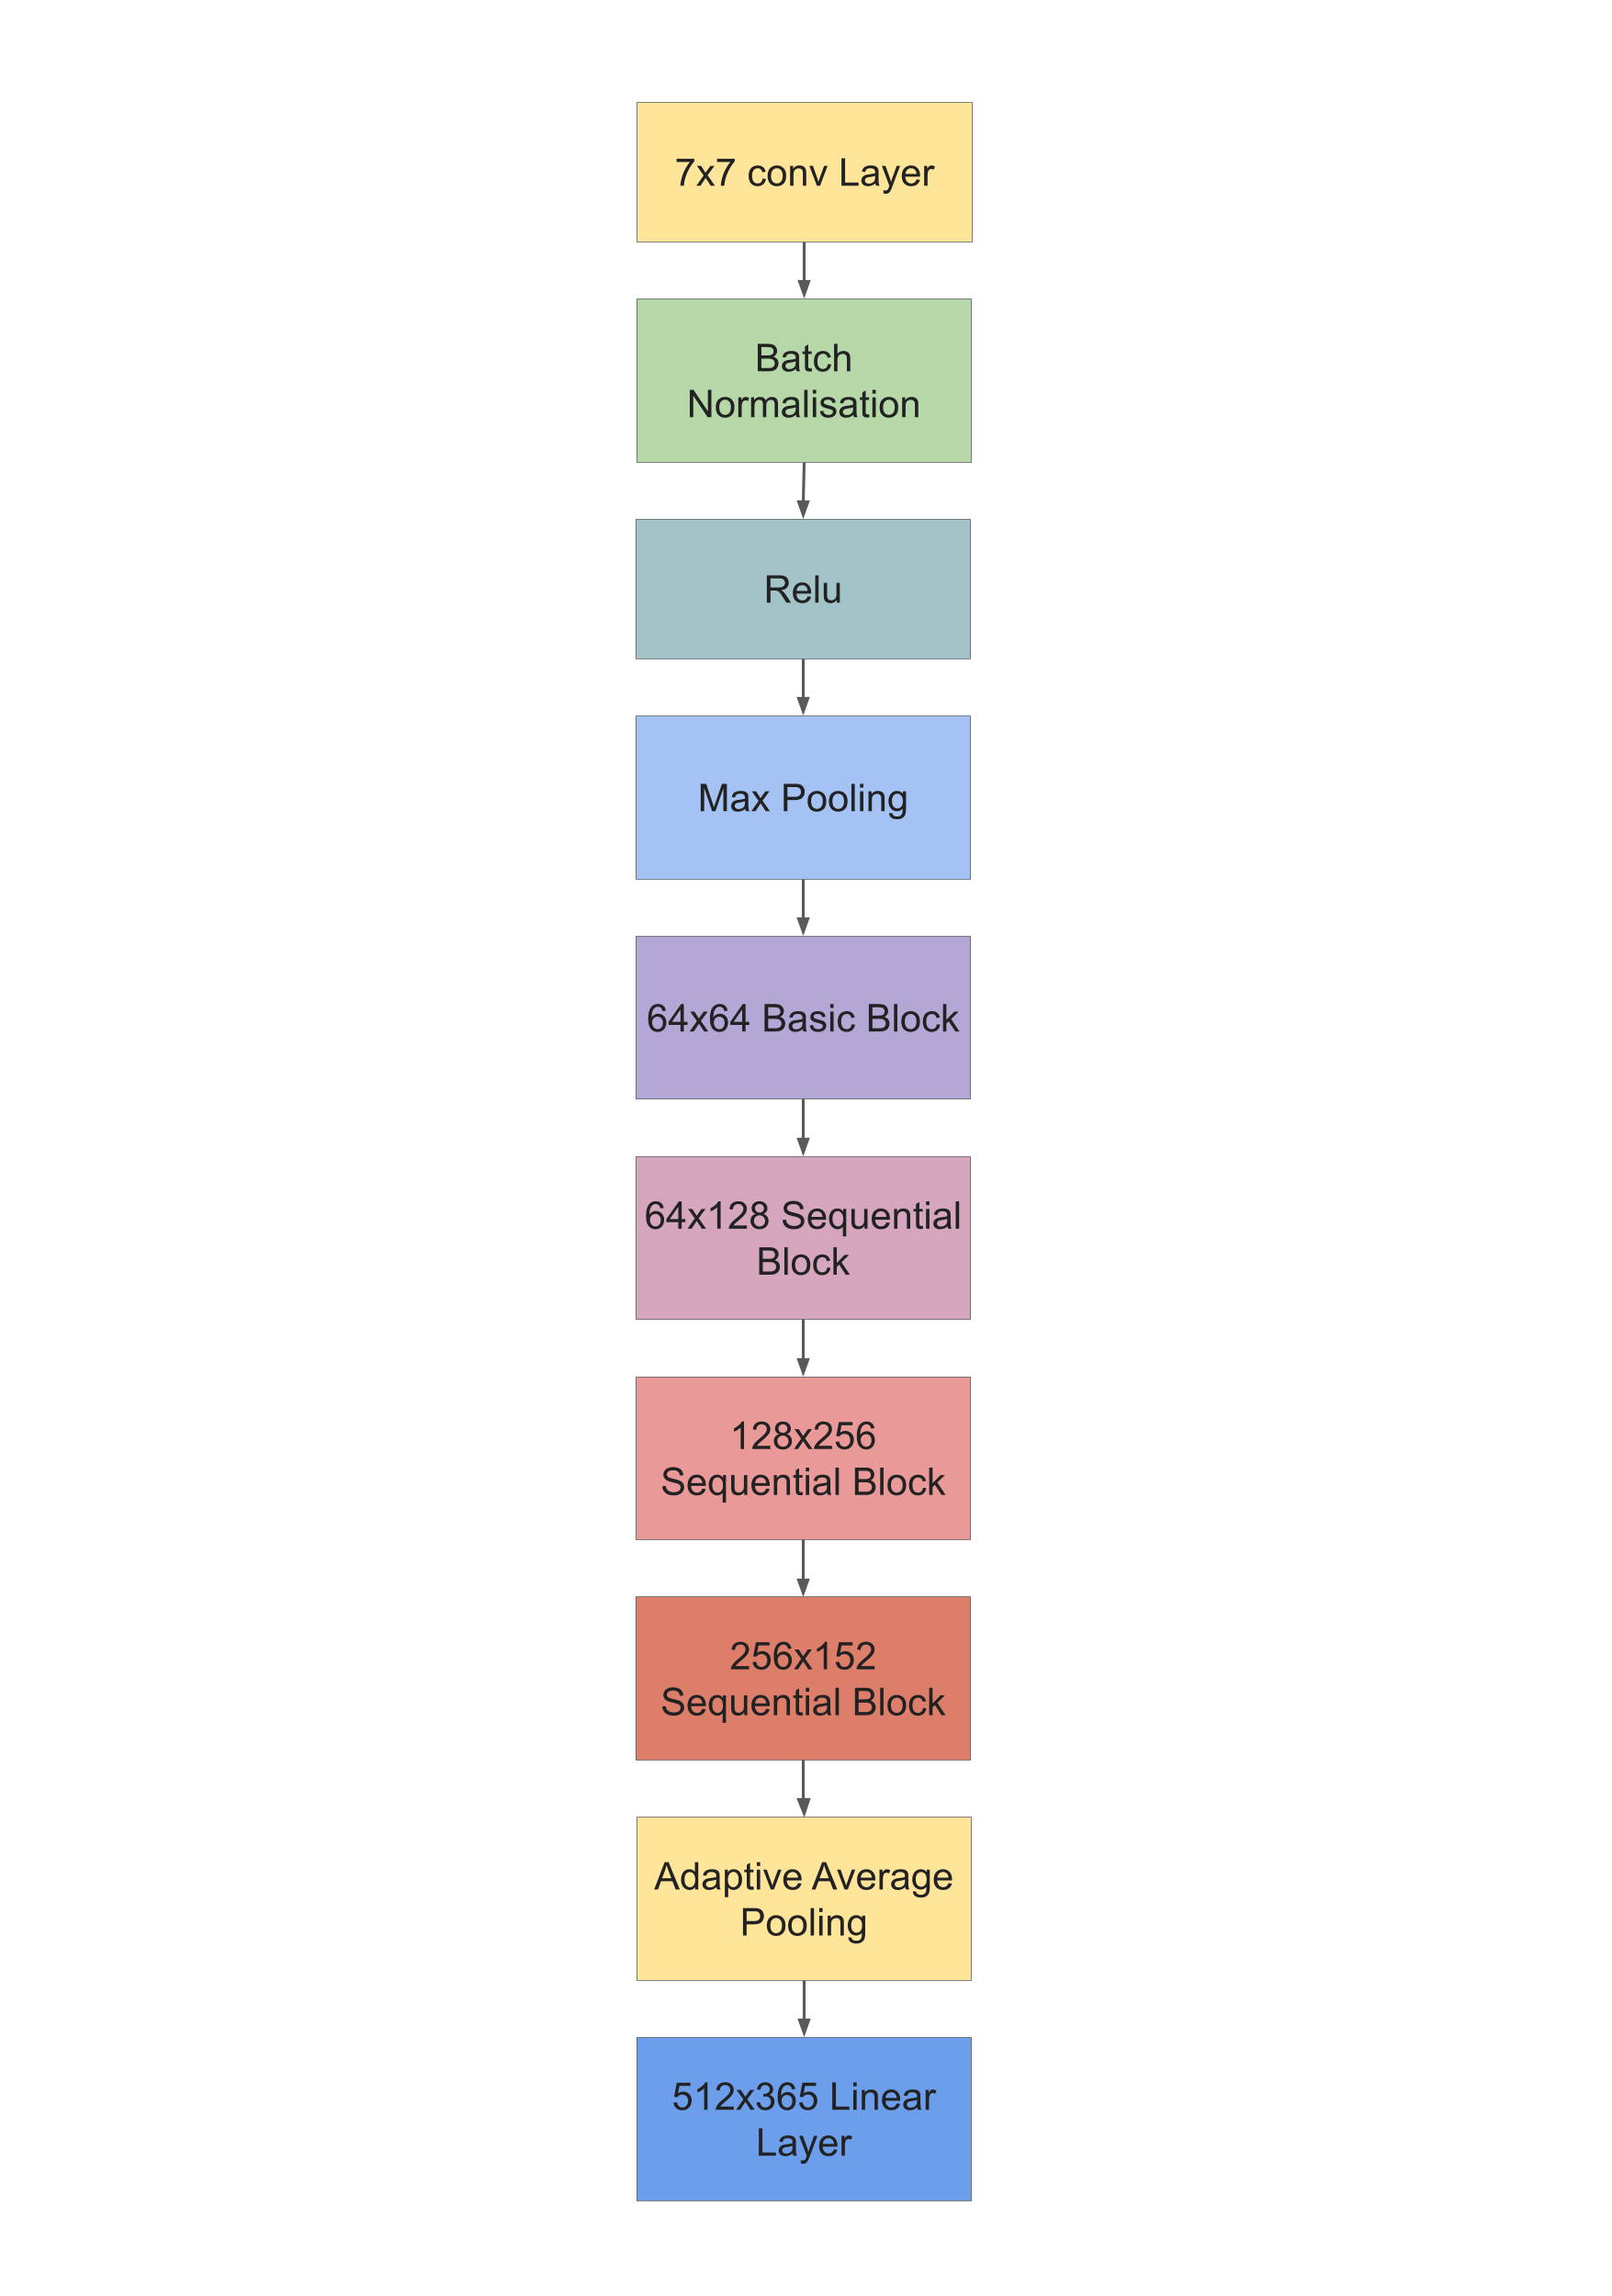
\includegraphics[width=0.8\textwidth]{Resnet.png}
\caption{Resnet 18 Architecture Summary}
\label{Resnet}
  \end{minipage}
\end{figure}

